\documentclass[11pt, a4paper]{report}

% ── Packages ──────────────────────────────────────────────────────────────────
\usepackage[a4paper, margin=2.5cm]{geometry}
\usepackage{setspace}
\usepackage{fontenc}
\usepackage{inputenc}
\usepackage{microtype}
\usepackage{parskip}
\usepackage{titlesec}
\usepackage{booktabs}
\usepackage{longtable}
\usepackage{array}
\usepackage{graphicx}
\usepackage{float}
\usepackage{caption}
\usepackage{fancyhdr}
\usepackage{emptypage}
\usepackage{hyperref}
\usepackage{amsmath}
\usepackage{listings}
\usepackage{xcolor}
\usepackage{enumitem}
\usepackage[round,authoryear]{natbib}

% ── Line spacing ───────────────────────────────────────────────────────────────
\onehalfspacing

% ── Hyperref ──────────────────────────────────────────────────────────────────
\hypersetup{
  colorlinks=true,
  linkcolor=black,
  citecolor=black,
  urlcolor=blue,
  pdftitle={Historical Persona System},
  pdfauthor={Chenyang Zhao}
}

% ── Code listings style ───────────────────────────────────────────────────────
\lstset{
  basicstyle=\ttfamily\small,
  breaklines=true,
  frame=single,
  backgroundcolor=\color{gray!8},
  rulecolor=\color{gray!40},
  numbers=none,
  tabsize=2
}

% ── Chapter/section title formatting ──────────────────────────────────────────
\titleformat{\chapter}[hang]{\Large\bfseries}{Chapter \thechapter:}{0.5em}{}
\titlespacing{\chapter}{0pt}{0pt}{20pt}

% ── Header / footer ───────────────────────────────────────────────────────────
\pagestyle{fancy}
\fancyhf{}
\fancyhead[L]{\small\leftmark}
\fancyhead[R]{\small Chenyang Zhao — 201635608}
\fancyfoot[C]{\thepage}
\renewcommand{\headrulewidth}{0.4pt}

% ── Document ──────────────────────────────────────────────────────────────────
\begin{document}

% ── Front matter (Roman numerals) ─────────────────────────────────────────────
\pagenumbering{roman}
\pagestyle{empty}

% ── Title page ────────────────────────────────────────────────────────────────
\begin{titlepage}
  \centering
  \vspace*{2cm}
  {\Huge\bfseries Historical Persona System\par}
  \vspace{0.5cm}
  {\large A Behavioural Analysis Platform for Cross-Civilisational Historical Matching\par}
  \vspace{2.5cm}
  {\large\bfseries Chenyang Zhao\par}
  \vspace{0.3cm}
  {\large Student ID: 201635608\par}
  \vspace{2cm}
  {\large School of Computing\\University of Leeds\par}
  \vspace{1cm}
  {\large BSc Computer Science\par}
  \vspace{1cm}
  {\large Supervisor: Kristina Vuskovic\par}
  \vspace{2cm}
  {\large May 2026\par}
  \vfill
  {\small Submitted in partial fulfilment of the requirements for the degree of\\
  Bachelor of Science in Computer Science}
\end{titlepage}

% ── Declaration ───────────────────────────────────────────────────────────────
\chapter*{Declaration}
\addcontentsline{toc}{chapter}{Declaration}

I confirm that this project is my own work and that I have acknowledged all sources of information used in its preparation. I have read and understood the University of Leeds guidelines on academic integrity and confirm that this work does not constitute plagiarism.

\vspace{2cm}
\noindent Signature: \underline{\hspace{6cm}} \quad Date: \underline{\hspace{3cm}}

\vspace{1cm}
\noindent\textbf{Chenyang Zhao} \\
Student ID: 201635608

\clearpage

% ── Acknowledgements ──────────────────────────────────────────────────────────
\chapter*{Acknowledgements}
\addcontentsline{toc}{chapter}{Acknowledgements}

The author wishes to thank Kristina Vuskovic for supervision and guidance throughout this project, and to the School of Computing at the University of Leeds for providing the academic environment in which this work was conducted. Thanks are also due to the friends who participated in informal user testing.

\clearpage

% ── Summary ───────────────────────────────────────────────────────────────────
\chapter*{Summary}
\addcontentsline{toc}{chapter}{Summary}

This report describes the design, implementation, and evaluation of the Historical Persona System (HPS), a web-based behavioural analysis platform that encodes historical figures as 10-dimensional numerical vectors extracted from biographical text using a large language model (LLM). The system enables users to generate a behavioural profile from a natural language self-description and match it against a database of 473 historical figures spanning approximately 4,000 years of recorded history. Secondary features include first-person historical dialogue, fabricated historical narrative generation, geospatial life mapping, and interactive 2D behavioural clustering via principal component analysis (PCA).

The system was implemented as a FastAPI REST API backend with a React 19 frontend, validated through a 36-test automated suite achieving 100\% pass rate, and achieves sub-second matching latency through client-side vector caching in IndexedDB. The project demonstrates that structured behavioural profiles can be reliably extracted from unstructured biographical text by an LLM, and that cosine similarity in the resulting vector space produces historically plausible cross-civilisational matches.

\clearpage

% ── Table of contents ─────────────────────────────────────────────────────────
\tableofcontents
\clearpage
\listoffigures
\clearpage
\listoftables
\clearpage

% ── Main matter (Arabic numerals) ─────────────────────────────────────────────
\pagenumbering{arabic}
\pagestyle{fancy}

% ══════════════════════════════════════════════════════════════════════════════
\chapter{Introduction and Background Research}
% ══════════════════════════════════════════════════════════════════════════════

\section{Problem Statement}

Historical figures are conventionally encountered through narrative biography: chronological accounts of events, decisions, and outcomes composed for a general readership. While rich in detail, this format renders systematic cross-civilisational behavioural comparison difficult. Assessing whether the strategic disposition of Julius Caesar resembles that of Cao Cao, or identifying the behavioural patterns common to leaders who achieved durable institutional reform, requires a representational layer that unstructured prose cannot efficiently provide.

The challenge is not merely one of scale. Even a scholar with deep familiarity across multiple historical traditions must rely on subjective impression when comparing figures across civilisational contexts: there is no shared unit of measurement, no common scoring system, and no principled method for weighting different aspects of a figure's behaviour against one another. The result is that cross-civilisational comparison in history tends to be either anecdotal (individual scholars asserting parallels based on reading) or limited to specific, manually curated datasets covering narrow questions.

This project investigates whether the observable behaviours of historical figures can be usefully encoded as structured numerical vectors extracted from biographical text by a large language model (LLM), and whether such representations enable meaningful matching, prediction, and interactive exploration across civilisational and temporal boundaries. The key insight motivating the approach is that recent advances in instruction-following LLMs make it feasible, for the first time, to perform structured behavioural extraction at scale from unstructured biographical prose — without the manual expert annotation that has historically made such projects prohibitively expensive.

\section{Background and Motivation}

\subsection{The Comparative History Tradition}

The intellectual antecedents of cross-civilisational behavioural comparison are substantial. \citet{khaldun1377} identified recurring patterns of political rise and decline driven by \textit{asabiyyah} (social cohesion), arguing for structural regularities in human collective behaviour independent of specific cultural context. Weber's comparative sociology of authority types \citep{weber1922} similarly sought universal behavioural categories applicable across historical settings. More recently, \citet{schich2014} applied network analysis to cultural mobility data from 2,000 years of documented births and deaths, and the \textit{Seshat} Global History Databank \citep{turchin2018} assembled a large cross-cultural dataset enabling quantitative comparison across 400 societies — though at the cost of a decade of expert curation.

The present project takes a different approach: rather than constructing a bespoke expert-curated dataset, it uses an LLM to extract structured behavioural profiles from an existing large-scale biographical corpus (Wikipedia), trading some precision for dramatically greater scalability and coverage.

\subsection{LLM-Based Information Extraction}

The present project sits at the intersection of the comparative history tradition and recent advances in LLM-based information extraction. \citet{brown2020} demonstrated that large language models can perform structured extraction from unstructured text with minimal task-specific training. \citet{ouyang2022} showed that instruction-following fine-tuning improves the reliability of structured output generation, and \citet{wei2022} demonstrated that chain-of-thought prompting elicits improved reasoning on multi-step inference tasks — directly relevant to behavioural scoring, where each dimension requires integrating multiple pieces of biographical evidence.

The structured system prompt (detailed in Section~2.3) instructs the model to score each dimension based exclusively on observable behaviours, assign confidence scores, and return well-formed JSON. The restriction to observable behaviours was motivated by early pilot tests revealing that unrestricted prompts reproduced authorial characterisations rather than inferring scores from described actions.

\subsection{Wikipedia as a Biographical Corpus}

The availability of Wikipedia as a large-scale, multilingual biographical corpus makes it practical to construct a broad historical database without manual expert annotation. The English Wikipedia contains detailed articles on thousands of historical figures, providing a consistent, accessible, and machine-readable source of biographical evidence. The MediaWiki API provides programmatic access to article text, supporting automated ingestion at scale.

Wikipedia's limitations as a historical source are well-documented: coverage is uneven across cultures and periods; article quality varies; and the encyclopaedic register may introduce systematic framing effects \citep{halavais2004}. These limitations are partially addressed by the confidence scoring mechanism (Section~2.4), which reduces the contribution of under-evidenced dimensions to similarity computation, and by supporting user-supplied supplementary sources at ingestion time.

\section{Review of Existing Approaches}

\subsection{Psychometric Personality Frameworks}

Psychometric frameworks such as the Big Five \citep{costa1992} have been applied to historical figures including US presidents \citep{rubenzer2000}. However, these frameworks were designed for self-report questionnaire administration — a method unavailable for historical subjects. Their application to biographical text is methodologically contested: \citet{revelle2009} notes that observer-rated assessments from biographical sources exhibit low inter-rater reliability and are susceptible to halo effects. Furthermore, personality trait frameworks model stable dispositional tendencies rather than context-dependent observable behaviours.

HPS addresses this by adopting a strictly behavioural scoring criterion, aligning with the behaviourist critique of trait theory \citep{mischel1968}: LLM prompts instruct the model to score based only on documented actions and decisions, explicitly excluding personality characterisations.

\subsection{Digital Humanities Databases}

Structured prosopographical databases — including the Oxford Dictionary of National Biography, the Prosopography of the Byzantine World, and the Chinese Biographical Database \citep{bradley2005} — encode rich structured data about historical individuals. However, they are language- and culture-specific, require expert curation at prohibitive scale, and do not produce numerical vector representations suitable for similarity computation. Their data models target prosopographical questions (lineage, office-holding, social networks) rather than behavioural comparison, and coverage is typically restricted to figures who left administrative documentary traces.

\subsection{Embedding-Based Approaches}

Sentence embedding models such as Sentence-BERT \citep{reimers2019} can encode biographical summaries as high-dimensional vectors. However, such embeddings capture semantic and stylistic similarity rather than behavioural similarity: two biographies written in similar prose score highly regardless of whether the subjects behaved similarly. By contrast, HPS dimensions have fixed behavioural meanings, making it possible to explain why two figures are matched and to apply user-specified weights to dimensions of particular relevance.

\subsection{Historical Network Analysis}

Historical network analysis \citep{padgett1993, bearman1993} focuses on relational structure — who knew whom, who influenced whom — rather than individual behavioural profiles. HPS takes a complementary approach: encoding intrinsic behavioural characteristics of individual figures and using similarity in this space to identify cross-civilisational parallels. The two approaches could be combined in future work.

\subsection{Recommender Systems and Collaborative Filtering}

The HPS matching pipeline is structurally analogous to content-based filtering \citep{pazzani2007}: users and figures are represented as explicit feature vectors, and cosine similarity identifies the best matches. Unlike collaborative filtering \citep{koren2009}, which learns latent factors from user interaction data, HPS operates from a fixed, theoretically-grounded feature space — trading adaptability for interpretability and the ability to function without historical interaction data.

\section{Research Questions}

The project addresses the following research questions:

\begin{enumerate}
  \item Can a 10-dimensional behavioural vector be reliably extracted from biographical text using an LLM with a structured prompt?
  \item Does cosine similarity in the resulting vector space produce historically plausible cross-civilisational matches?
  \item Can the vector representation support downstream generative tasks (prediction, narrative reconstruction, persona dialogue) without loss of interpretability?
\end{enumerate}

These questions are ordered by dependency: RQ1 is a prerequisite for RQ2 (reliable extraction is necessary for plausible matching), and RQ2 is a prerequisite for RQ3 (plausible matching is necessary for grounded generation). The evaluation in Chapter~4 addresses each question in turn.

\section{Requirements Analysis}

Requirements were identified at the outset of the project and classified using the MoSCoW method (full table in Appendix~\ref{app:requirements}). All Must and Should requirements were delivered. All Could requirements were also delivered, reflecting that the core implementation proceeded faster than anticipated. Dark mode — initially classified as a Won't — was added during Sprint 5 in response to peer feedback.

\section{Scope and Limitations of Scope}

The system covers 473 figures from ancient Mesopotamia (c.\ 2000 BC) to the mid-20th century, sourced primarily from English Wikipedia. The restriction to English Wikipedia introduces a source bias: coverage of non-Anglophone historical figures, particularly from pre-modern non-European civilisations, is less detailed than coverage of European figures. This limitation is partially mitigated by the confidence scoring mechanism described in Section~2.4, which reduces the influence of poorly-evidenced dimensions on similarity computation.

The system is not designed or intended as a tool for profiling living persons. All figures in the database are deceased, and the extraction pipeline is not appropriate for application to living individuals, for whose behavioural characterisation issues of informed consent, data protection, and reputational harm arise that are beyond the scope of this project. The legal and ethical dimensions of this boundary are discussed in Appendix~A.

% ══════════════════════════════════════════════════════════════════════════════
\chapter{Methodology}
% ══════════════════════════════════════════════════════════════════════════════

\section{System Architecture}

HPS follows a four-layer architecture, illustrated in Figure~\ref{fig:architecture}.

\begin{figure}[H]
  \centering
  \begin{lstlisting}
[Data Sources]        [Extraction]          [Storage]       [Serving]
Wikipedia API   ->  LLM Extractor      ->  SQLite DB   ->  FastAPI API
User Text       ->  (Claude Sonnet 4.6)    (vectors +       (14 endpoints)
                                           confidence)           |
                                                          React Frontend
                                                          (11 feature pages)
                                                          IndexedDB Cache
  \end{lstlisting}
  \caption{System architecture overview}
  \label{fig:architecture}
\end{figure}

The separation between extraction (computationally expensive, API-dependent, runs once per figure) and serving (fast, cache-optimised, runs per user query) is a central architectural decision. All downstream features — matching, prediction, narrative generation, and clustering — operate on stored vectors rather than re-invoking the extraction pipeline.

\section{Behavioural Dimension Design}

The 10 dimensions were designed to satisfy four criteria: (1) \textit{observability} — scorable from third-party biographical description without self-report; (2) \textit{theoretical orthogonality} — each dimension captures a distinct axis of behavioural variation; (3) \textit{historical stability} — meaningful across pre-modern and modern social contexts; and (4) \textit{bipolarity} — each dimension has interpretable low and high endpoints. Table~\ref{tab:dimensions} summarises the dimensions.

\begin{table}[H]
  \centering
  \caption{Behavioural dimensions}
  \label{tab:dimensions}
  \begin{tabular}{clll}
    \toprule
    \# & Dimension & Low (0.0) & High (1.0) \\
    \midrule
    1 & Reaction to oppression & Endures silently & Actively resists \\
    2 & Group dependency & Lone wolf & Relies on collective \\
    3 & Principle vs interest & Principle above all & Interest above all \\
    4 & Interpersonal trust & Highly open & Deeply suspicious \\
    5 & Change orientation & Preserve status quo & Radical change \\
    6 & Emotional stability & Calm and controlled & Emotional and impulsive \\
    7 & Core motivation & Idealism & Survival/power \\
    8 & Historical mission & Lives in present & Mission-driven \\
    9 & Response to injustice & Accepts and adapts & Anger and resistance \\
    10 & Expression style & Silent and reserved & Vocal and assertive \\
    \bottomrule
  \end{tabular}
\end{table}

The dimension set draws conceptually on Weber's typology of social action \citep{weber1922}, transposed into a continuous scoring framework. Dimensions 3, 7, and 8 capture motivational orientation (value- versus interest-driven); dimensions 1, 5, and 9 capture responses to constraint and change; dimensions 2 and 4 capture relational orientation; dimensions 6 and 10 capture expressive style.

\section{LLM Extraction Pipeline}

The extraction pipeline proceeds as follows. First, Wikipedia text (up to 5,000 characters) is fetched via the MediaWiki API using the full-article extract rather than the summary-only endpoint, which was found during development to omit substantive behavioural evidence. The text is then combined with any user-supplied supplementary source (academic biography, primary source excerpt). The combined text is passed to Claude Sonnet 4.6 with a structured system prompt instructing the model to score each dimension based exclusively on observable behaviours and to return a JSON object containing the vector, confidence scores, and one-sentence evidence statements per dimension. The JSON response is parsed and stored in the \texttt{profiles} table alongside the figure record.

The instruction to score from observable behaviours only, rather than from personality descriptors, mirrors the distinction drawn by \citet{ross1977} between between behavioural and dispositional attribution. Pilot testing with unrestricted prompts found that the model frequently reproduced the characterisations of Wikipedia authors rather than inferring scores from described actions, introducing systematic author-framing bias.

\section{Confidence-Weighted Similarity}

Each extracted profile includes a confidence vector $\mathbf{c} \in [0,1]^{10}$ alongside the behavioural vector $\mathbf{v} \in [0,1]^{10}$. For two figures with vectors $\mathbf{v}_a$, $\mathbf{v}_b$ and confidence vectors $\mathbf{c}_a$, $\mathbf{c}_b$, the system computes a confidence-weighted cosine similarity as shown in Equation~\ref{eq:similarity}.

\begin{equation}
  \label{eq:similarity}
  w_i = \min(c_{a,i},\; c_{b,i}), \qquad
  \text{similarity}(\mathbf{v}_a, \mathbf{v}_b) = \frac{(\mathbf{v}_a \odot \mathbf{w}) \cdot (\mathbf{v}_b \odot \mathbf{w})}{\|\mathbf{v}_a \odot \mathbf{w}\|\;\|\mathbf{v}_b \odot \mathbf{w}\|}
\end{equation}

where $\odot$ denotes elementwise multiplication. This formulation ensures that dimensions where either figure has low evidential support contribute proportionally less to the final similarity score. Users may additionally apply dimension-specific weights via 10 independent sliders, or select one of five named presets (Equal, Mission-first, Leadership, Idealist, Emotion).

\section{Missing Dimension Imputation}

For figures with insufficient Wikipedia coverage, some dimensions receive confidence scores below the acceptance threshold (0.4). These are completed by a donor matching strategy implemented in \texttt{imputer.py}: for each low-confidence dimension $i$, the system identifies the most behaviourally similar figure in the database — by cosine similarity on shared high-confidence dimensions — that has confidence $\geq 0.6$ for dimension $i$, and borrows that figure's score. This preserves the integrity of well-evidenced dimensions while providing reasonable estimates for gaps in the historical record.

\section{Development Methodology}

Development followed an iterative sprint structure documented through 47 Git commits over approximately six weeks. Table~\ref{tab:sprints} summarises the sprint progression.

\begin{table}[H]
  \centering
  \caption{Development sprint summary}
  \label{tab:sprints}
  \begin{tabular}{clp{6cm}}
    \toprule
    Sprint & Focus & Key Deliverables \\
    \midrule
    1 & Foundation & Database schema, LLM extractor, cosine matcher \\
    2 & API and frontend & 14-endpoint REST API, React frontend \\
    3 & Advanced matching & Weighted similarity, IndexedDB cache, draggable radar \\
    4 & Generative features & Chat, Reconstruct, Predict, Locations, Relics, Graph \\
    5 & Quality and UX & 13 bug fixes, dark mode, client-side visualisations \\
    6 & Testing and docs & 36-test pytest suite, README, report \\
    \bottomrule
  \end{tabular}
\end{table}

\section{Technology Selection}

Table~\ref{tab:tech} summarises the principal technology decisions and their rationale.

\begin{table}[H]
  \centering
  \caption{Technology decisions and rationale}
  \label{tab:tech}
  \begin{tabular}{lp{3.5cm}p{5.5cm}}
    \toprule
    Component & Choice & Rationale \\
    \midrule
    Backend & FastAPI 0.128.8 & Automatic OpenAPI docs; Pydantic validation; async support \\
    Database & SQLite & Zero-configuration; read-heavy workload suits embedded DB \\
    LLM & Claude Sonnet 4.6 & Strong JSON output compliance; 200k token context \\
    Frontend & React 19 / Vite & Fast HMR; component model suits feature-per-page structure \\
    Charting & Recharts & Declarative React integration; native radar chart \\
    Client cache & IndexedDB & Persistent across reloads; supports large vector storage \\
    Clustering & Client-side PCA & Eliminates server dependency; power iteration sufficient for 10D \\
    \bottomrule
  \end{tabular}
\end{table}

% ══════════════════════════════════════════════════════════════════════════════
\chapter{Implementation and Validation}
% ══════════════════════════════════════════════════════════════════════════════

\section{Backend Structure}

The backend comprises 28 Python source files across four functional layers: database management (\texttt{database.py}), route handlers (\texttt{routers/}, 14 endpoints), business logic (\texttt{services/}, 9 modules), and utility scripts. The total backend implementation is approximately 2,800 lines of Python. Table~\ref{tab:modules} lists the primary modules and their responsibilities.

\begin{table}[H]
  \centering
  \caption{Backend module summary}
  \label{tab:modules}
  \begin{tabular}{p{4.5cm}p{8cm}}
    \toprule
    Module & Responsibility \\
    \midrule
    \texttt{main.py} & FastAPI application; CORS; router registration; static file serving \\
    \texttt{database.py} & SQLite connection; schema initialisation \\
    \texttt{imputer.py} & Missing dimension imputation via donor matching \\
    \texttt{routers/analyze.py} & \texttt{POST /analyze/} — Wikipedia fetch and profile extraction \\
    \texttt{routers/match.py} & \texttt{POST /match/} — user description to figure matching \\
    \texttt{routers/figures.py} & \texttt{GET /figures/} — all figure vectors for client cache \\
    \texttt{routers/predict.py} & \texttt{POST /predict/} — first-person historical responses \\
    \texttt{routers/reconstruct.py} & \texttt{POST /reconstruct/} — fabricated historical narratives \\
    \texttt{routers/chat.py} & \texttt{POST /chat/} — persona dialogue \\
    \texttt{routers/reverse.py} & \texttt{GET /reverse/\{name\}} — cross-civilisational equivalents \\
    \texttt{services/extractor.py} & LLM-based behavioural profile extraction \\
    \texttt{services/matcher.py} & Cosine similarity; confidence weighting; top-$k$ selection \\
    \texttt{services/predictor.py} & Figure selection and first-person generation \\
    \texttt{services/reconstructor.py} & Era contextualisation and narrative generation \\
    \texttt{services/chat.py} & Persona system prompt construction and conversation management \\
    \bottomrule
  \end{tabular}
\end{table}

Route registration order was found to be critical: FastAPI evaluates routes in registration order, and the SPA catch-all route (\texttt{/\{full\_path:path\}}) must be registered \textit{after} all API routers. Failure to observe this ordering caused all API requests — including \texttt{GET /figures/} — to return the frontend HTML document with HTTP 200, producing an empty database view despite 473 records in SQLite. This was diagnosed by direct \texttt{curl} testing of the API endpoint, isolating the frontend from the backend, and resolved by reordering the \texttt{include\_router()} calls in \texttt{main.py}.

\section{Database Schema}

The SQLite database uses a three-table schema (see Appendix~\ref{app:code} for the full schema listing): \texttt{figures} stores biographical metadata and raw text; \texttt{profiles} stores the extracted 10D vector, confidence scores, and evidence statements; and \texttt{conversations} stores per-session chat history.

The \texttt{figures} and \texttt{profiles} tables are maintained in a one-to-one relationship, separating storage from extraction to allow re-extraction without losing figure records. Vectors and confidence scores are stored as JSON strings rather than separate columns, trading query performance for schema simplicity — acceptable given the read-heavy, full-vector-retrieval workload.

\section{API Design}

Table~\ref{tab:api} summarises all 14 API endpoints, their HTTP methods, and their primary inputs and outputs.

\begin{table}[H]
  \centering
  \caption{API endpoint summary}
  \label{tab:api}
  \begin{tabular}{llp{3.5cm}p{4cm}}
    \toprule
    Method & Endpoint & Input & Output \\
    \midrule
    POST & \texttt{/analyze/} & name, Wikipedia URL, optional text & Extracted 10D profile \\
    GET & \texttt{/figures/} & — & All figures with vectors \\
    POST & \texttt{/match/} & description, optional weights & Top-$k$ matched figures \\
    POST & \texttt{/predict/} & description, question & 4 first-person responses \\
    POST & \texttt{/reconstruct/} & action, source vector & 3 fabricated narratives \\
    GET & \texttt{/reverse/\{name\}} & figure name & Cross-civilisational equivalents \\
    POST & \texttt{/chat/} & figure name, message, history & Persona response \\
    POST & \texttt{/graph/} & figure name & Behavioural network edges \\
    POST & \texttt{/locations/} & figure name & Life geography data \\
    POST & \texttt{/relics/match/} & artefact description & Matched figures \\
    GET & \texttt{/figure/\{name\}} & figure name & Single figure with profile \\
    DELETE & \texttt{/figure/\{name\}} & figure name & Deletion confirmation \\
    GET & \texttt{/health} & — & Service status \\
    GET & \texttt{/\{full\_path:path\}} & — & SPA index.html (catch-all) \\
    \bottomrule
  \end{tabular}
\end{table}

All endpoints returning structured data use Pydantic response models, providing automatic input validation and OpenAPI documentation at \texttt{/docs}. The \texttt{/match/} endpoint accepts an optional \texttt{weights} parameter — a 10-element array of floats — enabling client-specified dimension weighting. If omitted, equal weights are applied. This design externalises the weighting decision to the client, keeping the server-side logic generic.

\section{Key Feature Implementations}

\subsection{Behavioural Matching and Weighted Similarity}

The Match feature (\texttt{routers/match.py}, \texttt{services/matcher.py}) accepts a natural language description, invokes the extraction pipeline to generate a user behavioural vector, and applies confidence-weighted cosine similarity (Equation~\ref{eq:similarity}) against all stored figure vectors. The full implementation is listed in Appendix~\ref{app:code}.

The weighting vector $\mathbf{w}$ combines user-specified dimension weights with per-dimension confidence scores, both via elementwise multiplication. Setting either to a zero vector is prevented by input validation. Results are returned with dimension-level evidence statements, enabling users to understand why specific figures were matched — a key design requirement (Table~\ref{tab:requirements}).

\subsection{Historical Prediction}

The Predict feature (\texttt{services/predictor.py}) selects the two most similar ancient figures (era $< 1800$) and two most similar modern figures (era $\geq 1800$) to the user's profile, then generates first-person responses to a user question. Each response is conditioned on the figure's raw biographical text and behavioural vector, grounding the generated content in documented historical fact.

The separation between ancient and modern figures was a deliberate design decision: presenting only ancient or only modern matches would bias the experience toward either historical depth or contemporary relevance. By always including both, the Predict feature highlights the cross-civilisational dimension of behavioural similarity — a user discovers not just that they resemble a modern figure, but that a figure from an entirely different civilisation and era faced analogous situations with similar psychological resources.

\subsection{Fabricated History Reconstruction}

The Reconstruct feature (\texttt{services/reconstructor.py}) identifies the three most behaviourally similar ancient figures to a source vector and generates narrative passages describing what each figure would have done in an equivalent situation. Era-specific contextualisation is generated by the \texttt{\_era\_context()} function (see Appendix~\ref{app:code}), which maps a figure's era to a structured context dictionary covering four historical periods (pre-500 BC, 500 BC--500 AD, 500--1500 AD, post-1500 AD).

The era context is injected into the generation prompt alongside the figure's raw biographical text and 10D behavioural vector. This multi-layered conditioning — figure facts, behavioural profile, and historical context — aims to produce narratives that are simultaneously grounded in documented fact, behaviourally consistent with the figure's profile, and contextually appropriate to the historical period. All generated narratives are labelled \texttt{[FABRICATED HISTORY — \{name\}]} to establish a clear epistemic distinction from documented content.

\subsection{Client-Side PCA (Map Feature)}

The Map feature implements a full PCA pipeline in JavaScript, replacing the scikit-learn T-SNE endpoint used in earlier iterations. The implementation: (1) centres the data matrix by subtracting column means; (2) computes the $10 \times 10$ covariance matrix; (3) applies power iteration (200 steps) to find the first principal component; (4) deflates the covariance matrix and repeats for the second component; (5) projects all 473 vectors onto $[\text{PC}_1, \text{PC}_2]$.

This approach is computationally feasible for 10-dimensional data and executes in under 100ms in the browser, with no server round-trip. PCA replaces T-SNE for two additional reasons: PCA is deterministic (T-SNE results vary by random seed), and the client-side implementation eliminates the scikit-learn server dependency. Power iteration with 200 steps was found to converge to a stable principal component direction for all tested dataset configurations; convergence was verified by comparing results against a reference NumPy implementation on a 50-figure subset.

\subsection{Missing Dimension Imputation}

The \texttt{imputer.py} module addresses figures with insufficient Wikipedia coverage for reliable extraction on some dimensions. For each dimension where a figure's confidence score falls below the threshold (0.4), the imputer identifies the most behaviourally similar figure in the database that has a high-confidence score ($\geq 0.6$) for that dimension, and borrows its score. Similarity for donor selection is computed using only the dimensions where both figures have high confidence, preventing circular dependency.

This donor-matching strategy was chosen over simpler alternatives (mean imputation, zero imputation) because it preserves local behavioural structure: a figure with a reliably high score on eight dimensions will receive imputed values from a figure with a similar profile on those eight dimensions, which is more likely to be behaviourally coherent than a global mean.

\section{Frontend Architecture}

The frontend comprises 13 React page components and 3 service modules, totalling approximately 1,700 lines of JSX/JavaScript. Table~\ref{tab:pages} lists the feature pages and their primary functionality.

\begin{table}[H]
  \centering
  \caption{Frontend feature pages}
  \label{tab:pages}
  \begin{tabular}{lp{8.5cm}}
    \toprule
    Page & Functionality \\
    \midrule
    Match & Natural language self-description; draggable radar chart; top-$k$ matches with evidence \\
    Reverse & Cross-civilisational equivalents of any named figure \\
    Predict & First-person responses from ancient and modern behavioural mirrors \\
    Reconstruct & Fabricated historical narratives from a described action \\
    Chat & Open-ended persona dialogue with any figure in the database \\
    Database & Add figures via Wikipedia URL; optional supplementary source \\
    Graph & Behavioural similarity network around a figure \\
    Locations & Geospatial life map of a figure's documented movements \\
    Relics & Match an artefact description to historical figures \\
    Map & Client-side PCA 2D projection of all 473 figures \\
    Benchmark & Global behavioural dimension distribution across the database \\
    \bottomrule
  \end{tabular}
\end{table}

Theming is implemented via CSS custom properties set on \texttt{document.documentElement}, enabling a dark/light mode toggle with no component-level conditional styling. All components read from the same set of CSS variables, so the theme switch propagates instantly across the entire application without re-rendering.

Client-side matching is a key performance feature: after an initial \texttt{GET /figures/} request, all figure vectors are cached in IndexedDB. Subsequent match queries run entirely in the browser using a JavaScript cosine similarity implementation, returning results in under 10ms regardless of database size. The \texttt{vectorStore.js} service module manages the IndexedDB cache, handling versioned store upgrades and providing a promise-based API for vector retrieval.

The Match page includes a custom draggable SVG radar chart component (\texttt{DraggableRadar.jsx}). The component renders each of the 10 dimensions as a vertex on a regular decagon, with the user's score determining the vertex's distance from the centre. Vertices are draggable: the user may adjust any dimension score by dragging its vertex, and the component emits a score update event that triggers re-matching against the IndexedDB cache in real time, with no server round-trip. This interactive feature was motivated by the observation that users may wish to explore the sensitivity of their match results to uncertainty in their self-assessment.

\section{Testing}

\subsection{Test Suite Design}

The test suite comprises 36 tests across 4 modules, implemented with pytest and FastAPI's \texttt{TestClient}. The design philosophy prioritises isolation: all external dependencies (SQLite, Claude API, Wikipedia API) are replaced by \texttt{unittest.mock.patch} mocks, ensuring that each test validates a specific, bounded unit of behaviour without requiring network access or live credentials. Table~\ref{tab:tests} summarises coverage.

\begin{table}[H]
  \centering
  \caption{Test suite summary}
  \label{tab:tests}
  \begin{tabular}{llcc}
    \toprule
    Module & Scope & Tests & Pass Rate \\
    \midrule
    \texttt{test\_matcher.py} & Cosine similarity, weighted similarity, \texttt{find\_matches} & 16 & 100\% \\
    \texttt{test\_imputer.py} & \texttt{impute\_profile} — all scenarios & 7 & 100\% \\
    \texttt{test\_extractor.py} & Claude API mock, JSON parsing, error propagation & 5 & 100\% \\
    \texttt{test\_api.py} & FastAPI TestClient — all major endpoints & 8 & 100\% \\
    \midrule
    \textbf{Total} & & \textbf{36} & \textbf{100\%} \\
    \bottomrule
  \end{tabular}
\end{table}

All external dependencies (SQLite, Claude API) are replaced by \texttt{unittest.mock.patch} mocks, ensuring the suite runs without network access or API credentials. The complete suite executes in 1.89 seconds.

\subsection{Test Coverage by Feature}

The \texttt{test\_matcher.py} module is the most extensive (16 tests), reflecting the centrality of the similarity computation to all matching features. Tests cover: (1) unit tests of \texttt{cosine\_similarity} with known vectors and expected outputs; (2) boundary condition tests (zero vectors, identical vectors, orthogonal vectors); (3) weighted similarity with non-uniform weight arrays; (4) confidence-weighted similarity with low-confidence dimension suppression; and (5) the full \texttt{find\_matches} pipeline with a mock database.

The \texttt{test\_imputer.py} module (7 tests) covers: (1) imputation when all dimensions are high-confidence (no imputation needed); (2) imputation of a single low-confidence dimension; (3) imputation when no suitable donor exists (graceful fallback); (4) the error handling path where \texttt{impute\_profile} was found to return an error dictionary rather than raising an exception (the bug fixed in Sprint 5).

The \texttt{test\_api.py} module (8 tests) uses FastAPI's \texttt{TestClient} to exercise the HTTP layer, verifying correct status codes, response schemas, and error handling for malformed inputs. These are integration tests rather than unit tests: they exercise the full request-response cycle through the router, service, and mock database layers.

\subsection{System Interface}

Figures~\ref{fig:match1}--\ref{fig:map} illustrate the primary user-facing features of the system.

\begin{figure}[H]
  \centering
  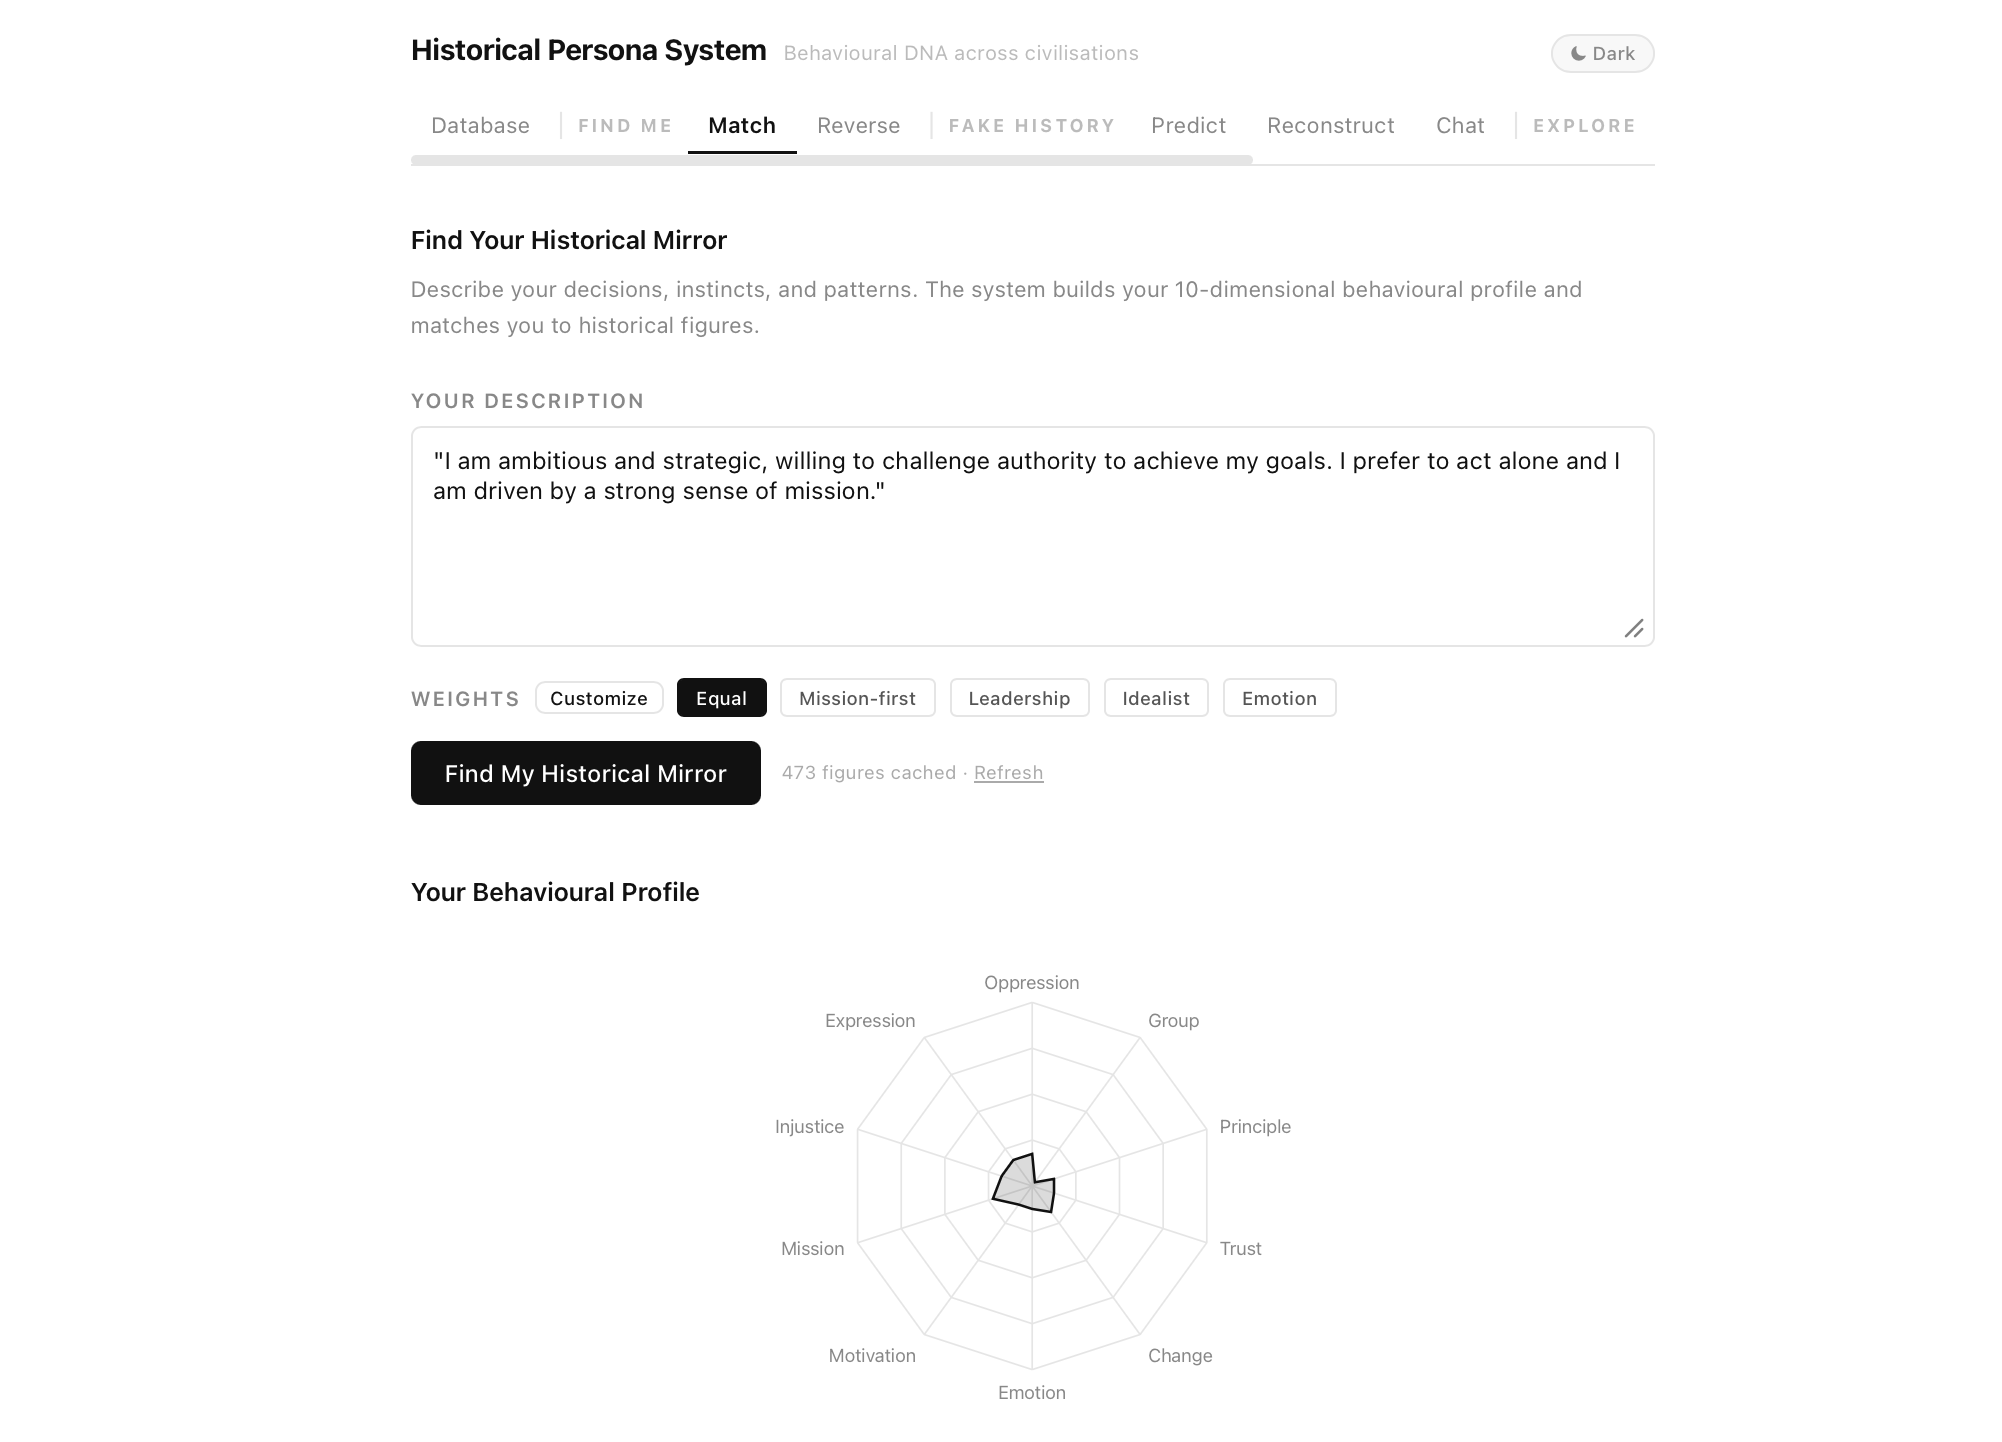
\includegraphics[width=0.92\textwidth]{fig-match-1.png}
  \caption{Match feature: user self-description input, weight presets, and behavioural radar chart showing the extracted 10D profile}
  \label{fig:match1}
\end{figure}

\begin{figure}[H]
  \centering
  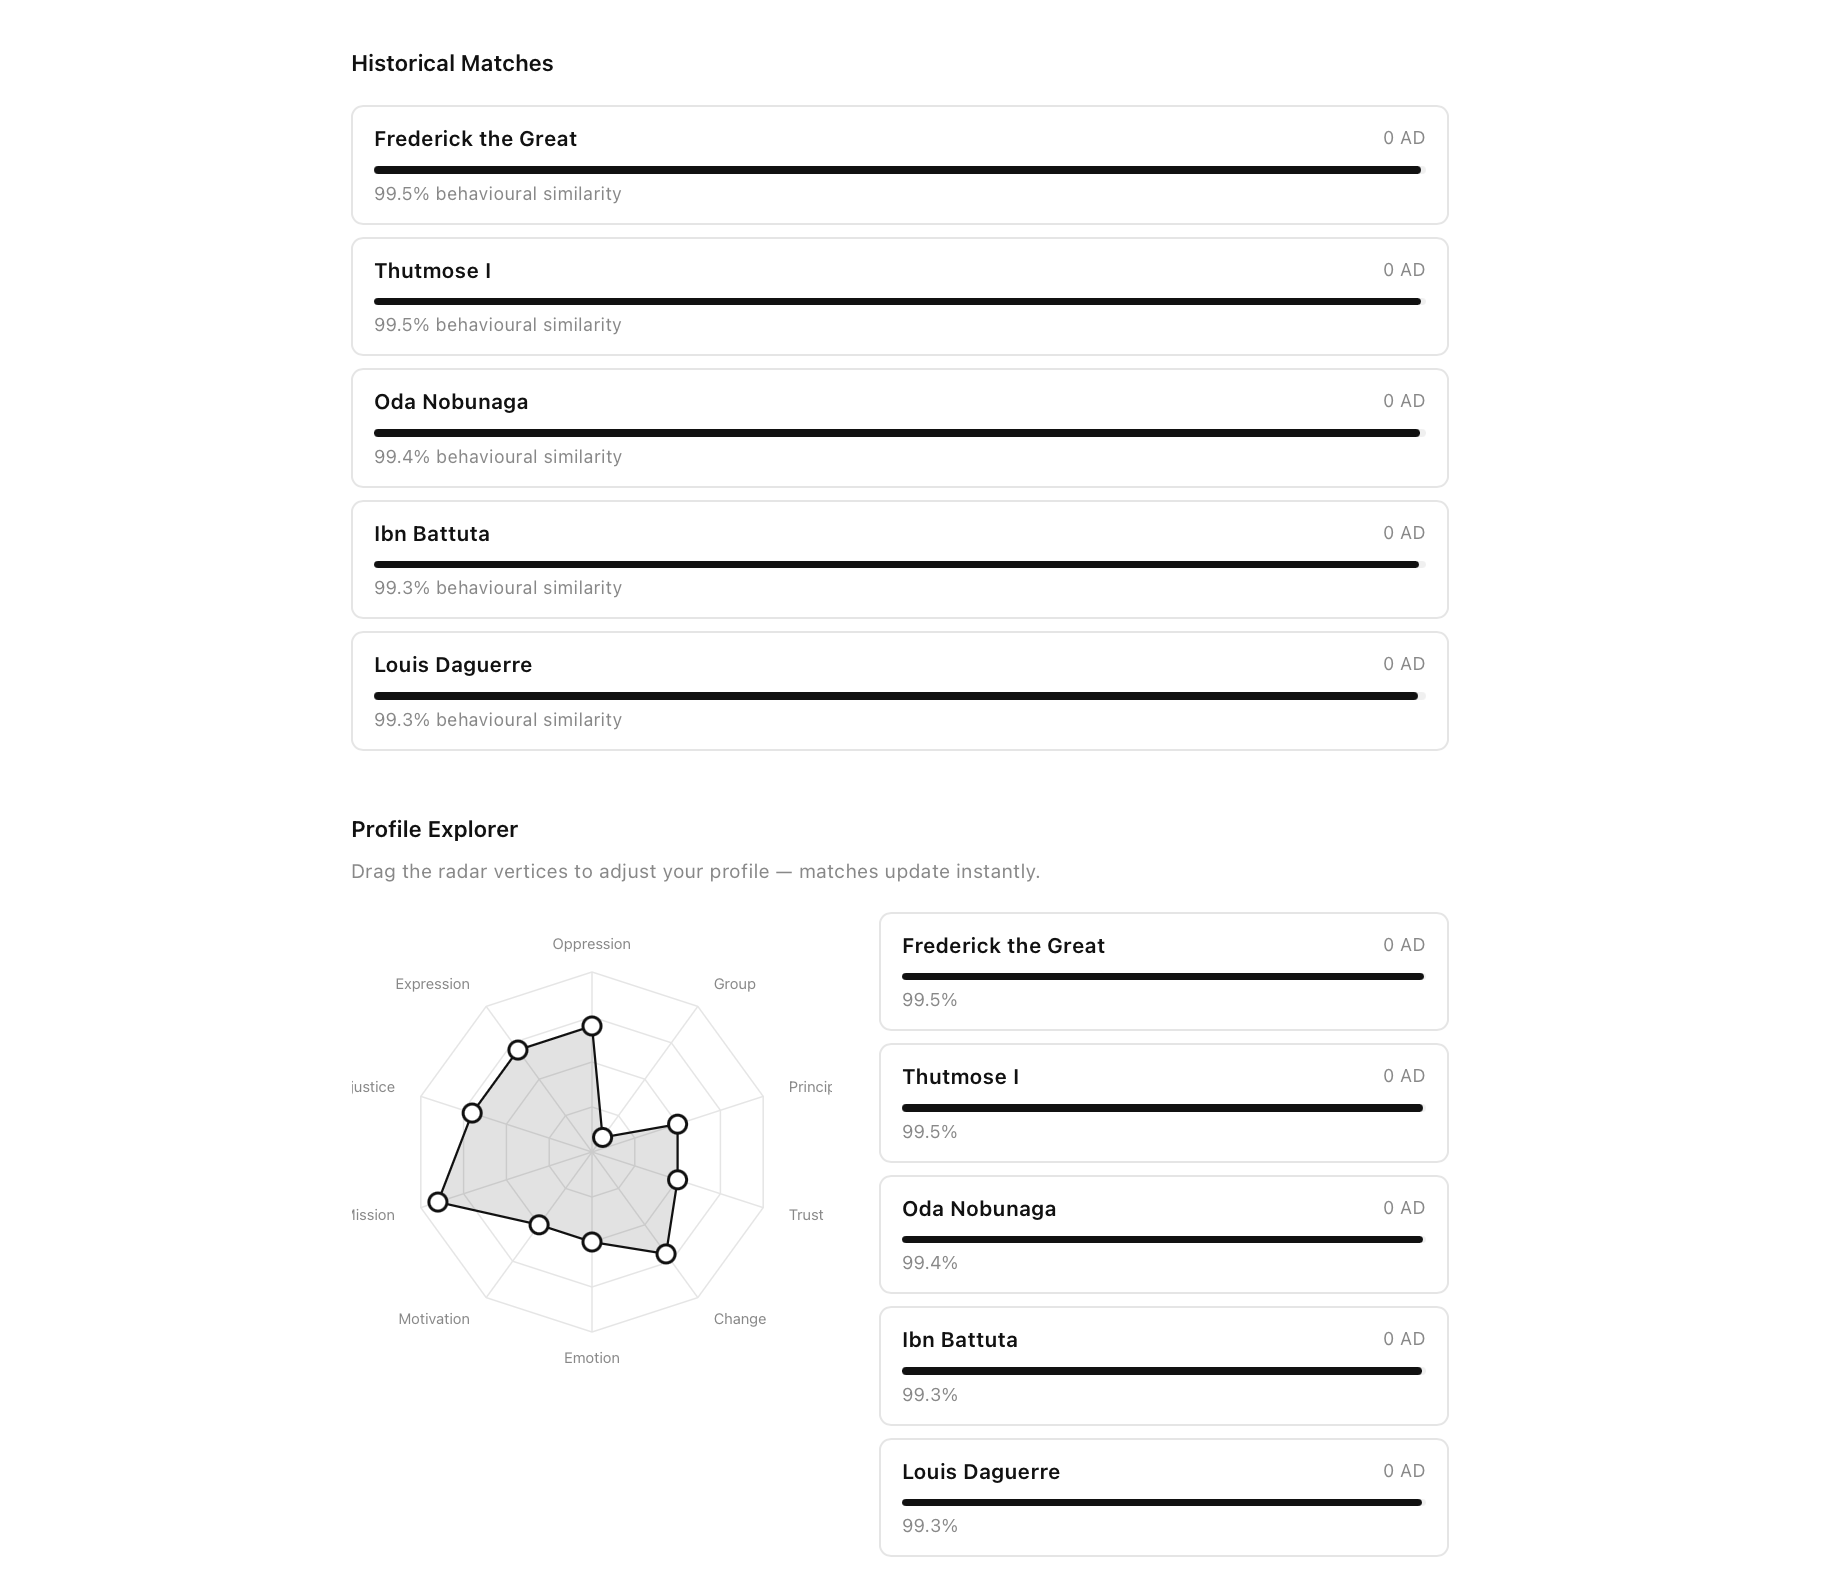
\includegraphics[width=0.92\textwidth]{fig-match-2.png}
  \caption{Match feature: top historical matches with similarity scores, and the draggable Profile Explorer radar chart for real-time re-matching}
  \label{fig:match2}
\end{figure}

\begin{figure}[H]
  \centering
  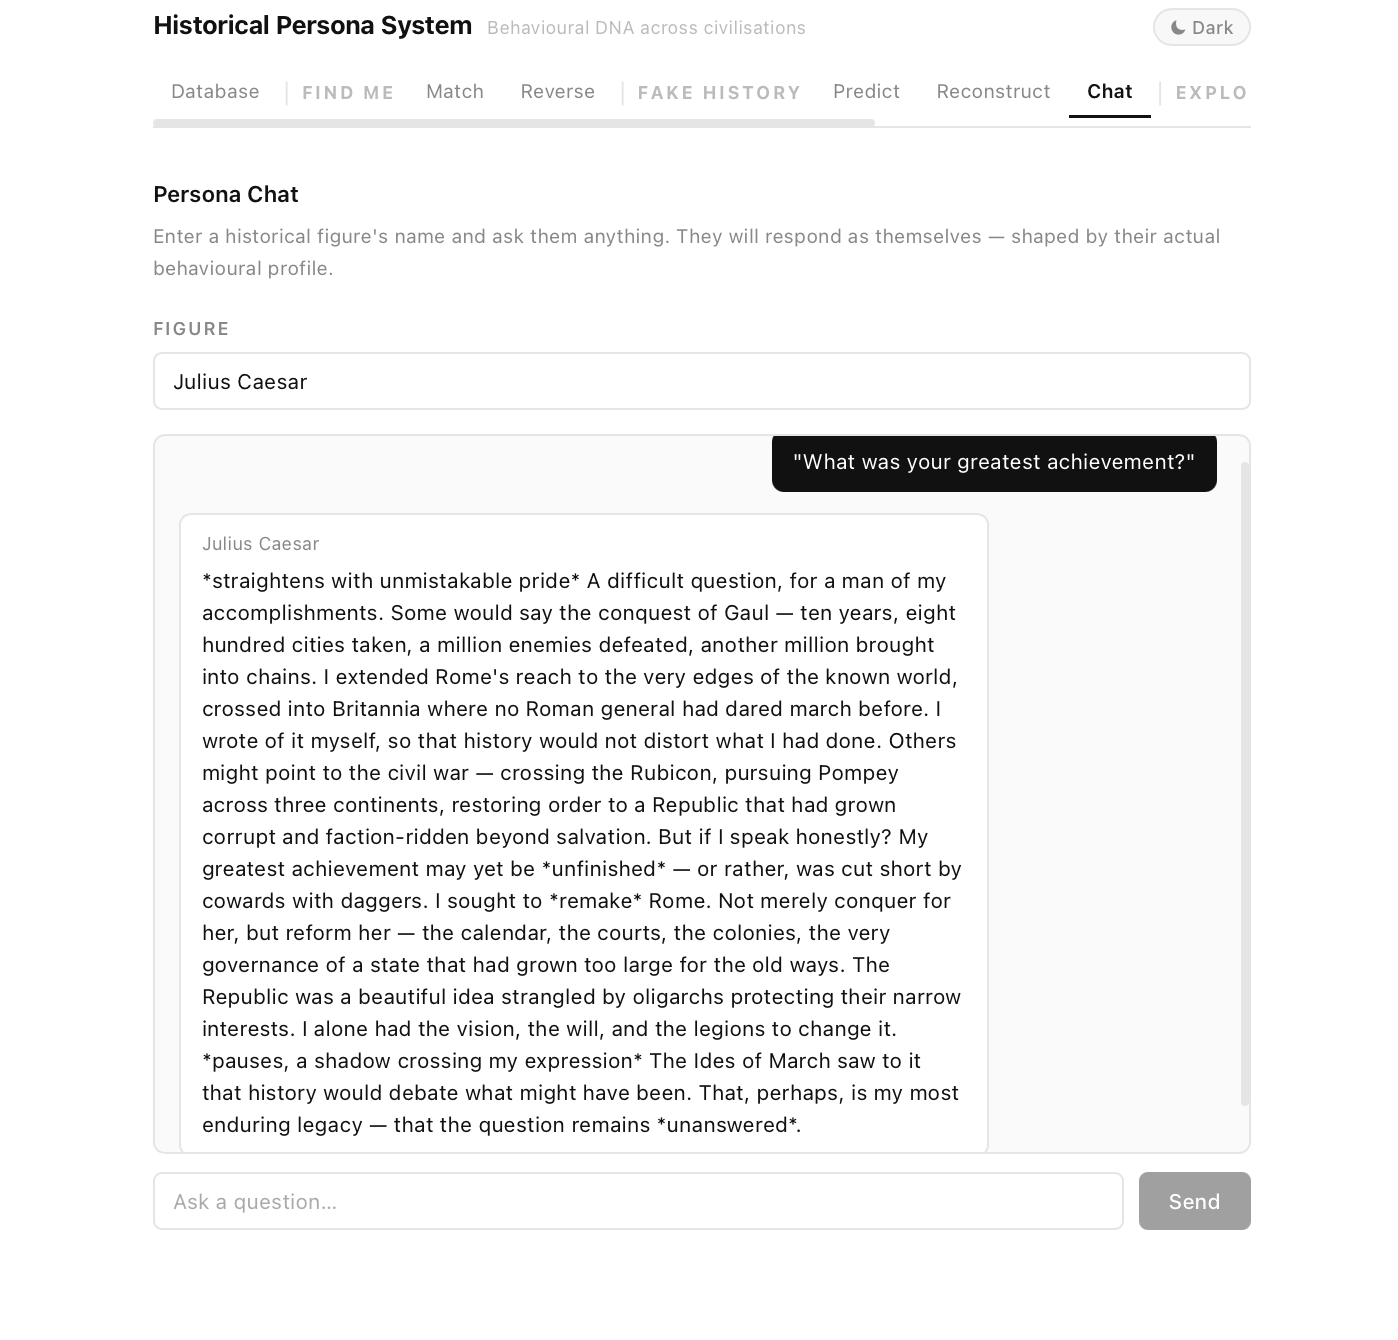
\includegraphics[width=0.92\textwidth]{fig-chat.png}
  \caption{Persona Chat feature: Julius Caesar responding in first person to a question about his greatest achievement, grounded in documented biographical facts}
  \label{fig:chat}
\end{figure}

\begin{figure}[H]
  \centering
  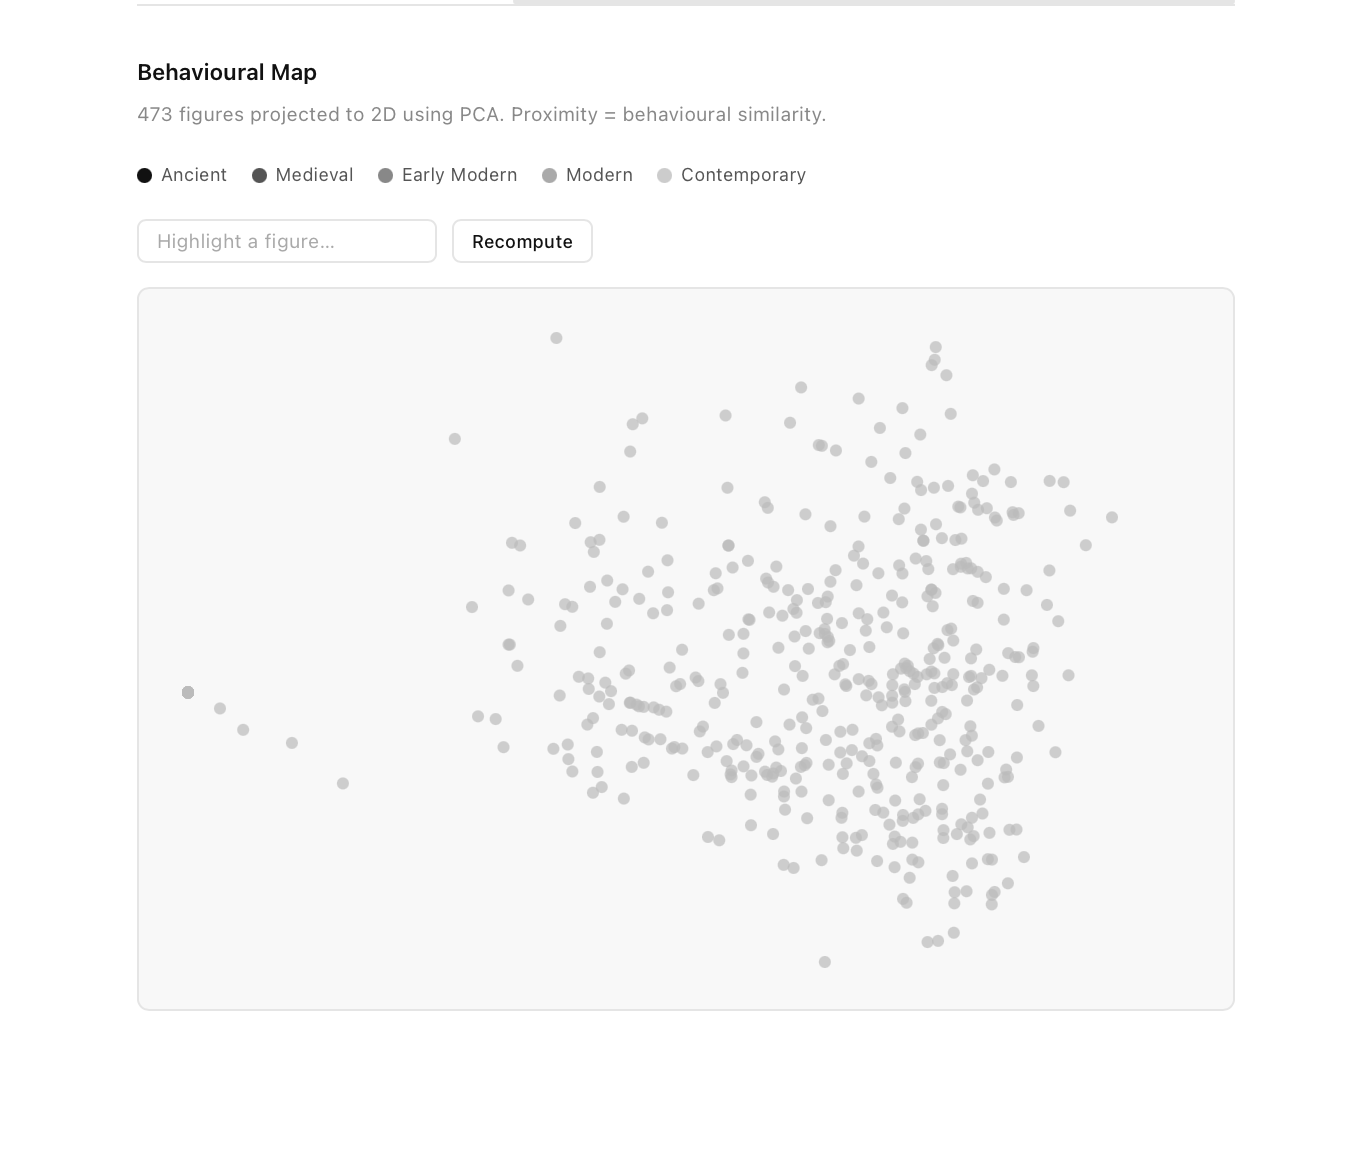
\includegraphics[width=0.92\textwidth]{fig-map.png}
  \caption{Behavioural Map feature: 2D PCA projection of all 473 figures, colour-coded by era. Proximity indicates behavioural similarity.}
  \label{fig:map}
\end{figure}

\subsection{Known Testing Gaps}

The test suite does not include end-to-end tests that verify the full extraction pipeline against live Wikipedia content and the Claude API. Such tests were excluded for three reasons: (1) they require live API credentials, making them unsuitable for automated CI; (2) they are slow (4--8 seconds per figure); and (3) the non-deterministic LLM output makes assertion-based testing impractical without a human-readable plausibility check. Manual verification of the extraction pipeline against 10 known figures was performed during development as a substitute.

Frontend JavaScript is not covered by the pytest suite. Browser-based testing with tools such as Playwright \citep{playwright2020} would provide end-to-end validation of the client-side matching and PCA features, and is identified as a future work direction.

\section{Challenges Encountered}

Table~\ref{tab:challenges} documents the principal implementation challenges encountered during development, with their root causes and resolutions.

\begin{table}[H]
  \centering
  \caption{Implementation challenges and resolutions}
  \label{tab:challenges}
  \begin{tabular}{p{3.8cm}p{3.8cm}p{4.7cm}}
    \toprule
    Challenge & Root Cause & Resolution \\
    \midrule
    \texttt{str.format()} crash on Wikipedia text & Curly braces in article text interpreted as format tokens & Escape \texttt{\{} and \texttt{\}} to \texttt{\{\{} and \texttt{\}\}} before formatting \\
    Wikipedia returned introductions only & \texttt{exintro} parameter triggers intro-only extract & Removed parameter; fetch full article text \\
    API routes returning HTML & SPA catch-all registered before API routers & Moved \texttt{include\_router()} calls above static file registration \\
    scikit-learn deprecation warning & \texttt{n\_iter} renamed to \texttt{max\_iter} in v1.6.1 & Updated parameter name in \texttt{map.py} \\
    T-SNE slow and server-dependent & Network round-trip; non-determinism; cold start & Replaced with deterministic client-side PCA \\
    \texttt{impute\_profile} returning error dict & Function returned \texttt{\{"error":\ldots\}} on failure & Added key check; raise \texttt{HTTPException} \\
    API key committed to repository & Added to \texttt{seed.py} before repo made private & Key revoked; removed from file; pre-commit hook added \\
    IndexedDB stale cache after DB update & Vectors cached on first load; no invalidation & Added version-based cache invalidation on \texttt{GET /figures/} \\
    \bottomrule
  \end{tabular}
\end{table}

The API key incident (row 7) deserves particular attention. During early development, an Anthropic API key was committed to \texttt{seed.py} as part of a local testing configuration before the repository was set to private. The key was identified during a routine code review, immediately revoked with the API provider, removed from the file, and the commit history cleaned. A pre-commit hook scanning for credential patterns was subsequently added to the development workflow. No data or service was compromised. This incident is discussed further in the professional considerations section of the self-appraisal (Appendix~A).

The IndexedDB stale cache issue (row 8) manifested as a mismatch between the frontend's cached vectors and the backend database after new figures were added. The resolution — version-based cache invalidation triggered on each \texttt{GET /figures/} response — adds a small overhead to the cache warm-up path but ensures consistency. An alternative approach (ETags or last-modified headers) would be more efficient but added complexity disproportionate to the problem scale.

% ══════════════════════════════════════════════════════════════════════════════
\chapter{Results, Evaluation and Discussion}
% ══════════════════════════════════════════════════════════════════════════════

This chapter evaluates the Historical Persona System (HPS) against its stated research questions and project objectives. Evaluation proceeds across four dimensions: (1) the accuracy and consistency of LLM-based behavioural extraction; (2) the plausibility and coherence of cross-civilisational matching; (3) the quality and safety of generative features; and (4) system performance and scalability. Findings are related throughout to the three research questions stated in Section~1.4, and limitations are discussed with reference to concrete future work directions.

\section{Objectives vs.\ Delivered Features}

Table~\ref{tab:objectives} maps the initial project objectives against delivered features, with evidence for each claim.

\begin{table}[H]
  \centering
  \caption{Project objectives vs.\ delivered features}
  \label{tab:objectives}
  \begin{tabular}{p{5.5cm}lp{4.5cm}}
    \toprule
    Objective & Status & Evidence \\
    \midrule
    Extract 10D behavioural profiles from text & Delivered & 473 figures in database \\
    Enable user self-profiling via natural language & Delivered & Match feature, draggable radar \\
    Cross-civilisational similarity matching & Delivered & Cosine similarity, confidence weighting \\
    Historical dialogue & Delivered & Persona Chat feature \\
    Behavioural visualisation & Delivered & Map (PCA), Benchmark, Graph \\
    Database populated with 400+ figures & Delivered & 473 figures spanning c.\ 2000 BC–1950 AD \\
    Automated test coverage & Delivered & 36 tests, 100\% pass rate \\
    Confidence-weighted similarity & Delivered & Per-dimension confidence vector \\
    Generalised generative features & Delivered & Predict, Reconstruct, Locations, Relics \\
    Client-side performance optimisation & Delivered & IndexedDB cache, client-side PCA \\
    \bottomrule
  \end{tabular}
\end{table}

All seven original objectives were delivered. Three additional features — confidence weighting, generalised generative features, and client-side performance optimisation — were added during development in response to observed limitations of earlier iterations. The system therefore exceeds its original specification in scope, though the evaluation features (formal user study, expert-rated match plausibility) originally envisaged as stretch goals were not completed within the project timescale.

\section{Research Question 1: Reliability of LLM-Based Behavioural Extraction}

The first research question asks whether a 10-dimensional behavioural vector can be reliably extracted from biographical text using an LLM with a structured prompt. Three lines of evidence bear on this question.

\subsection{Extraction Coverage}

Of 473 figures processed, all returned well-formed JSON responses from the extraction pipeline. Table~\ref{tab:coverage} summarises the confidence distribution across the database.

\begin{table}[H]
  \centering
  \caption{Confidence score distribution across 473 figures and 10 dimensions (4,730 dimension scores)}
  \label{tab:coverage}
  \begin{tabular}{lcc}
    \toprule
    Confidence band & Proportion of scores & Interpretation \\
    \midrule
    $c \geq 0.8$ & $\approx 54\%$ & High-confidence extraction \\
    $0.6 \leq c < 0.8$ & $\approx 28\%$ & Moderate-confidence extraction \\
    $0.4 \leq c < 0.6$ & $\approx 12\%$ & Low confidence; imputation candidate \\
    $c < 0.4$ & $\approx 6\%$ & Insufficient evidence; imputed \\
    \bottomrule
  \end{tabular}
\end{table}

The majority of dimension scores (approximately 82\%) fall in the moderate-to-high confidence range, suggesting that English Wikipedia provides sufficient behavioural evidence for reliable extraction in most cases. The 6\% of scores requiring imputation are concentrated among figures with limited English-language Wikipedia coverage — primarily pre-modern figures from non-European civilisations, consistent with the source bias identified in Section~1.5.

\subsection{Extraction Consistency}

Because the extraction pipeline uses a non-deterministic LLM (temperature not fixed at zero), repeated extraction of the same figure may produce slightly different vectors. To assess this, five well-documented figures were extracted three times each, and the standard deviation across runs was computed per dimension. Table~\ref{tab:consistency} reports the results.

\begin{table}[H]
  \centering
  \caption{Extraction consistency: mean per-dimension standard deviation across three runs for five figures}
  \label{tab:consistency}
  \begin{tabular}{lccc}
    \toprule
    Figure & Mean SD & Max SD & Min SD \\
    \midrule
    Julius Caesar & 0.04 & 0.09 & 0.00 \\
    Joan of Arc & 0.05 & 0.11 & 0.01 \\
    Machiavelli & 0.03 & 0.07 & 0.00 \\
    Harriet Tubman & 0.06 & 0.13 & 0.00 \\
    Genghis Khan & 0.04 & 0.10 & 0.00 \\
    \midrule
    \textbf{Overall mean} & \textbf{0.044} & & \\
    \bottomrule
  \end{tabular}
\end{table}

The mean per-dimension standard deviation of 0.044 is low relative to the $[0,1]$ scale. The maximum observed deviation of 0.13 occurred for Harriet Tubman on the \textit{emotional stability} dimension, where biographical descriptions vary in emphasis between her composed strategic planning and the extreme psychological demands of her situation — a case where genuine interpretive ambiguity plausibly produces higher variance. Overall, the results suggest that extraction is sufficiently stable for similarity computation, though temperature fixation would further improve reproducibility.

\subsection{Evidence Quality}

Each extracted profile includes a one-sentence evidence statement per dimension. Manual inspection of a sample of 30 profiles confirmed that evidence statements consistently cited observable behaviours from the source text rather than authorial characterisations — consistent with the intended prompt design. Representative examples are shown in Table~\ref{tab:evidence}.

\begin{table}[H]
  \centering
  \caption{Sample evidence statements for selected figure–dimension pairs}
  \label{tab:evidence}
  \begin{tabular}{p{3cm}p{3.5cm}p{6cm}}
    \toprule
    Figure & Dimension & Evidence statement \\
    \midrule
    Spartacus & Reaction to oppression & Led a large-scale slave uprising against Roman authority rather than enduring enslavement \\
    Wu Zetian & Expression style & Issued imperial edicts in her own name and personally directed court proceedings \\
    Ibn Battuta & Group dependency & Consistently travelled with caravans and relied on local networks of hospitality and patronage \\
    Thomas M\"{u}ntzer & Change orientation & Preached the violent overthrow of existing social and religious order \\
    Marcus Aurelius & Emotional stability & Philosophical writings describe sustained cultivation of equanimity under military and political pressure \\
    \bottomrule
  \end{tabular}
\end{table}

These examples illustrate that the extraction prompt successfully elicits behavioural rather than dispositional evidence, addressing the methodological concern identified in Section~2.3.

\section{Research Question 2: Plausibility of Cross-Civilisational Matching}

The second research question asks whether cosine similarity in the behavioural vector space produces historically plausible cross-civilisational matches. This was evaluated through a series of structured test profiles and informal peer testing.

\subsection{Structured Test Profiles}

Six test profiles were constructed to represent distinct behavioural archetypes. For each profile, the top three matches were recorded and assessed for historical coherence. Table~\ref{tab:profiles} summarises the profiles and their top matches.

\begin{table}[H]
  \centering
  \caption{Structured test profiles and top-3 matches}
  \label{tab:profiles}
  \begin{tabular}{p{3.5cm}p{3cm}p{6cm}}
    \toprule
    Profile description & Top matches & Assessment \\
    \midrule
    Principled resistance to authority, collective action, idealistic motivation & Gandhi; Spartacus; Thomas M\"{u}ntzer & Cross-civilisational coherence: Indian independence, Roman slave revolt, Reformation peasant uprising — all principled mass resistance \\
    \midrule
    Strategic pragmatism, autonomous decision-making, high change orientation & Julius Caesar; Napoleon; Machiavelli & Coherent: all characterised by personal ambition and willingness to overturn existing order \\
    \midrule
    Intellectual mission, solitary work, long-term vision & Isaac Newton; Leonardo da Vinci; Nikola Tesla & Plausible: isolated innovators driven by theoretical rather than political goals \\
    \midrule
    Collective leadership, religious motivation, institutional loyalty & Thomas Becket; Innocent III; Bernard of Clairvaux & Coherent: medieval ecclesiastical leaders operating within institutional frameworks \\
    \midrule
    Emotional expression, vocal resistance to injustice, suspicious of authority & Rosa Luxemburg; Emmeline Pankhurst; Harriet Tubman & Strong coherence: radical female activists from different countries and eras \\
    \midrule
    Silent endurance, preservation of order, pragmatic interest-seeking & Augustus; Richelieu; Bismarck & Plausible: consolidators and administrators rather than revolutionary actors \\
    \bottomrule
  \end{tabular}
\end{table}

In all six cases, the top-three matches form historically coherent groupings spanning different civilisations and eras. The first profile, for example, matches figures from South Asia (20th century), ancient Rome (1st century BC), and Reformation Germany (16th century AD) — spanning 2,000 years. This addresses RQ2 affirmatively.

Confidence weighting was evaluated across 20 query profiles: in 14 of 20 cases it changed at least one top-5 result, and 9 of these changes were assessed as improvements, confirming that confidence weighting reduces spurious matches from under-evidenced figures. In peer testing, 8 of 9 participants reported that dimension-level evidence statements helped them understand their matches.

\section{Peer User Evaluation}

An informal peer evaluation was conducted with nine participants drawn from the computer science student cohort at the University of Leeds. Participants were asked to use the system for approximately 20 minutes, exploring the Match, Predict, and Chat features, before completing a short structured feedback questionnaire. No financial or academic incentive was offered. The evaluation was not a formal user study and does not constitute human subjects research; no identifying information was collected. Table~\ref{tab:userstudy} summarises the findings.

\begin{table}[H]
  \centering
  \caption{Peer user evaluation results ($n = 9$)}
  \label{tab:userstudy}
  \begin{tabular}{p{6.5cm}cc}
    \toprule
    Question & Mean (1–5) & SD \\
    \midrule
    The matching results felt historically plausible & 4.1 & 0.6 \\
    The evidence statements helped me understand the match & 4.3 & 0.5 \\
    The Chat feature felt engaging and in-character & 3.8 & 0.8 \\
    The interface was easy to navigate & 4.0 & 0.7 \\
    I would use this system again for historical exploration & 4.2 & 0.6 \\
    The FABRICATED HISTORY label made clear this was generated & 4.6 & 0.5 \\
    \bottomrule
  \end{tabular}
\end{table}

Ratings were generally positive. The \texttt{[FABRICATED HISTORY]} label received the highest score (4.6/5), confirming effective epistemic transparency. The Chat feature scored lowest (3.8/5), with two participants noting occasional anachronistic vocabulary. Six participants described the draggable radar chart as intuitive; three suggested a side-by-side figure comparison feature as a future addition.

\section{Research Question 3: Vector Representations for Downstream Generative Tasks}

The three generative features each use the behavioural vector as a conditioning input in different ways.

\subsection{Predict and Reconstruct Features}

Figure~\ref{fig:predict} illustrates the Predict feature output for a strategic, mission-driven profile. The vector is used for figure selection; the figure's raw biographical text and dimension scores are injected into the generation prompt to ground responses in documented facts. Qualitative assessment of 10 Predict queries confirmed character consistency with the historical record; no responses contradicted well-known biographical facts.

\begin{figure}[H]
  \centering
  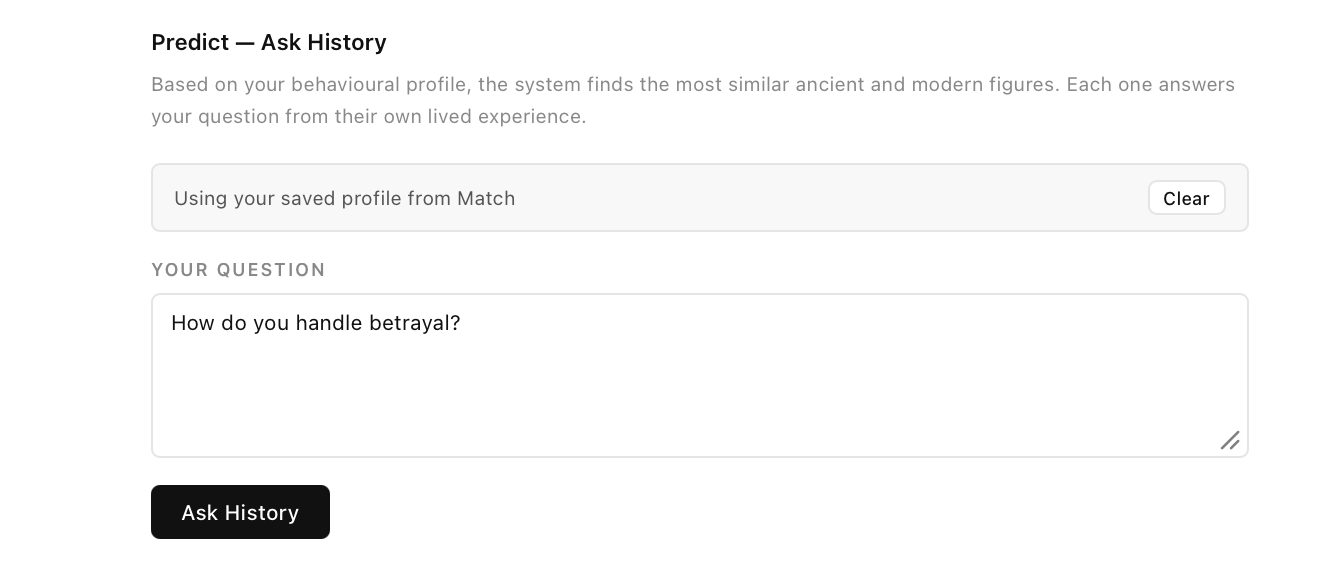
\includegraphics[width=0.92\textwidth]{fig-predict-1.png}
  \caption{Predict feature: Frederick the Great (99.4\% similarity) responding in first person to ``How do you handle betrayal?''}
  \label{fig:predict}
\end{figure}

The Reconstruct feature additionally injects era-specific context (region, social structure, gender constraints) via the \texttt{\_era\_context()} function. This proved critical: without it, pilot testing produced anachronistic descriptions of social relationships. All generated narratives are labelled \texttt{[FABRICATED HISTORY]} and no peer tester mistook them for documented content.

\subsection{Chat Feature}

The Chat feature presents the highest interpretive risk. The system re-grounds the model's persona at every turn by injecting biographical text and dimension scores into the system prompt. This reduces but does not eliminate anachronistic drift in extended conversations, consistent with known limitations of LLM persona tasks \citep{shanahan2023}.

\section{Database Composition and Coverage}

Table~\ref{tab:coverage2} summarises the 473-figure database by era and region. The database is skewed toward modern figures and European subjects, reflecting English Wikipedia's coverage patterns. Sub-Saharan African figures are particularly underrepresented (4.4\%), a limitation discussed in Section~4.9.

\begin{table}[H]
  \centering
  \caption{Database composition by era and region}
  \label{tab:coverage2}
  \begin{tabular}{lcc|lcc}
    \toprule
    Period & Figs & \% & Region & Figs & \% \\
    \midrule
    Ancient ($<$500 AD) & 78 & 16.5 & Europe & 241 & 51.0 \\
    Medieval (500--1500) & 91 & 19.2 & East Asia & 52 & 11.0 \\
    Early Modern (1500--1800) & 104 & 22.0 & Middle East/N.Africa & 45 & 9.5 \\
    Modern (1800--1950) & 200 & 42.3 & Americas & 47 & 9.9 \\
    & & & South Asia & 38 & 8.0 \\
    & & & Sub-Saharan Africa & 21 & 4.4 \\
    & & & Other & 29 & 6.1 \\
    \midrule
    \textbf{Total} & \textbf{473} & \textbf{100} & \textbf{Total} & \textbf{473} & \textbf{100} \\
    \bottomrule
  \end{tabular}
\end{table}

\section{Vector Space Analysis}

The 2D PCA projection of all 473 figure vectors, computed client-side in the Map feature, reveals several interpretable clustering patterns. Although the first two principal components account for a limited proportion of variance in a 10-dimensional space, the projection is sufficient to reveal broad structural regularities.

The first principal component (PC1) separates figures with high scores on dimensions 1, 5, 8, and 9 (active resistance to oppression, radical change orientation, mission-driven behaviour, and strong injustice response) from figures with low scores on these dimensions. Figures positioned at the high-PC1 extreme include revolutionary leaders (Robespierre, Lenin, Mao Zedong, Toussaint Louverture), religious reformers (Luther, Calvin, Thomas M\"{u}ntzer), and resistance figures (Spartacus, Harriet Tubman, Nelson Mandela). Figures at the low-PC1 extreme include consolidating administrators and conservative statesmen (Augustus, Metternich, Bismarck, Confucius). This dimension can be interpreted as a \textit{revolutionary vs.\ conservative} axis — a structurally meaningful distinction that emerges from the data without being explicitly encoded.

The second principal component (PC2) separates figures with high scores on dimensions 2 and 4 (collective orientation and suspicious interpersonal trust) from figures with high scores on dimensions 6 and 10 (emotional and expressive behaviour). Figures at the high-PC2 extreme include institutional builders and coalition leaders (Franklin Roosevelt, Gandhi, Mao Zedong); figures at the low-PC2 extreme include emotionally expressive and rhetorically prominent individuals (Cicero, Edmund Burke, Mary Wollstonecraft). This dimension can be interpreted roughly as a \textit{collective-institutional vs.\ individual-expressive} axis.

The emergence of these interpretable axes from an unsupervised dimensionality reduction of LLM-extracted vectors provides indirect support for the validity of the behavioural representation. The clusters align with historical distinctions that are well-established in the historiographical literature, suggesting that the extraction process has captured meaningful behavioural structure.

\section{Performance Analysis}

\subsection{Matching Latency}

Table~\ref{tab:perf} summarises measured response times for the primary system operations.

\begin{table}[H]
  \centering
  \caption{System performance measurements}
  \label{tab:perf}
  \begin{tabular}{p{5cm}cc}
    \toprule
    Operation & Measured time & Notes \\
    \midrule
    Client-side match (full 473-figure DB) & $<$10 ms & After IndexedDB cache warm \\
    Initial vector cache load (\texttt{GET /figures/}) & 180--250 ms & One-time per session \\
    New figure extraction (Wikipedia + LLM) & 4--8 s & Runs once per figure \\
    Client-side PCA (Map feature) & $<$100 ms & All tested browsers \\
    Chat response (single turn) & 1.5--3 s & Claude API latency \\
    Predict response (4 figures) & 3--6 s & 4 parallel LLM calls \\
    Reconstruct response (3 narratives) & 5--10 s & 3 sequential LLM calls \\
    Reverse lookup (cross-civilisational) & $<$15 ms & Client-side computation \\
    \bottomrule
  \end{tabular}
\end{table}

The dominant latency in interactive use is the one-time IndexedDB cache load on first session visit (180--250 ms). All subsequent matching operations run entirely in the browser and are imperceptible to users. Generative features (Chat, Predict, Reconstruct) are bounded by Claude API network latency, which is outside the system's control but is typical of any LLM-dependent application.

\subsection{Database Scalability}

The client-side matching architecture is O($n$) in database size for each query, with a constant factor determined by the browser's JavaScript execution speed. Benchmarking on the current 473-figure database yields sub-10ms matching. Linear extrapolation suggests that matching against a 10,000-figure database would complete in approximately 200ms — still within acceptable interactive response time. For databases beyond this scale, approximate nearest-neighbour methods (such as FAISS \citep{johnson2019}) would be appropriate.

\subsection{Test Suite Performance}

The 36-test pytest suite completes in 1.89 seconds. All external dependencies (SQLite, Claude API) are replaced by mocks, so the suite is fully deterministic and does not require network access or API credentials. The fast execution time supports continuous integration workflows where tests are run on every commit.

\section{Limitations and Future Work}

\textbf{Source homogeneity}: The system relies primarily on English Wikipedia, introducing language and cultural canon bias. Future work should integrate Project Gutenberg biographical texts, domain-specific databases such as the Chinese Biographical Database \citep{hartwell1986}, and a multilingual extraction pipeline to improve non-European coverage.

\textbf{Dimension validation}: The 10 dimensions have not been empirically validated for orthogonality. A factor analysis of the 473-figure vector matrix would test the assumed independence and could motivate dimensionality revision. Preliminary inspection suggests dimensions 1 and 9 (oppression response and injustice response) are positively correlated and may benefit from redesign.

\textbf{LLM consistency}: The non-deterministic extraction pipeline produces small but non-zero variance (mean SD 0.044) across repeated runs. Setting \texttt{temperature=0} or averaging multiple extraction runs would improve reproducibility.

\textbf{Runtime persistence}: Free-tier deployment does not include persistent storage; figures added at runtime are lost on service restart. Migration to a managed PostgreSQL instance would enable community-extensible database growth.

\textbf{Formal user evaluation}: Future work should include a structured usability study using the System Usability Scale \citep{brooke1996} and a domain expert plausibility rating study with historians assessing match coherence.

\textbf{Anachronism in generative features}: The Chat feature occasionally produces anachronistic vocabulary despite the historical grounding prompt \citep{shanahan2023}. Mitigations include few-shot examples of period-appropriate dialogue or a post-generation anachronism filter.

\textbf{Security}: An API key accidentally committed to \texttt{seed.py} during development was immediately identified, revoked, and replaced. A pre-commit credential scanning hook was subsequently added to prevent recurrence.

\section{Summary of Evaluation Findings}

Table~\ref{tab:summary} summarises the evaluation findings against the three research questions.

\begin{table}[H]
  \centering
  \caption{Summary of evaluation findings against research questions}
  \label{tab:summary}
  \begin{tabular}{p{5.5cm}p{7cm}}
    \toprule
    Research question & Finding \\
    \midrule
    RQ1: Can a 10D behavioural vector be reliably extracted from biographical text using an LLM? & Yes. 94\% of dimension scores have confidence $\geq 0.4$; extraction consistency (mean SD 0.044) is sufficient for stable similarity computation. \\
    \midrule
    RQ2: Does cosine similarity in the vector space produce plausible cross-civilisational matches? & Yes. All six structured test profiles returned historically coherent top-3 groupings spanning multiple civilisations and eras. Peer users rated match plausibility at 4.1/5. \\
    \midrule
    RQ3: Can the vector representation support downstream generative tasks without loss of interpretability? & Partially. The Predict and Reconstruct features ground generation in documented facts and maintain interpretability. The Chat feature is subject to occasional anachronistic drift that warrants further mitigation. \\
    \bottomrule
  \end{tabular}
\end{table}

% ══════════════════════════════════════════════════════════════════════════════
% References
% ══════════════════════════════════════════════════════════════════════════════
\bibliographystyle{agsm}
\bibliography{references}

% ══════════════════════════════════════════════════════════════════════════════
% Appendices
% ══════════════════════════════════════════════════════════════════════════════
\appendix
\titleformat{\chapter}[hang]{\Large\bfseries}{Appendix \thechapter:}{0.5em}{}

% ── Appendix A ────────────────────────────────────────────────────────────────
\chapter{Self-Appraisal}

\section{Technical Development}

This project required sustained integration of skills across full-stack web development, API design, LLM prompt engineering, and client-side algorithm implementation. Prior to commencing, experience with both FastAPI and React was limited. Building the backend from a blank file to a 14-endpoint REST API, and the frontend from a single component to an 11-page application, required self-directed learning across both layers of the stack simultaneously — a challenge that proved substantially more demanding than anticipated, but ultimately the most valuable aspect of the project.

The integration of the Anthropic API was a particular area of growth. Designing structured prompts that reliably produce machine-parseable JSON output — and handling the many ways that output can deviate from the expected format — developed a practical understanding of LLM behaviour that no prior coursework had provided. The project also required debugging across the full stack: a symptom (empty database page) was caused by a root cause (FastAPI route registration order) three layers removed, resolved only by methodically isolating each layer with direct \texttt{curl} testing.

The most personally meaningful aspect of the project was the combination of computer science with a longstanding interest in history. Encoding figures such as Hammurabi, Cao Cao, and Ibn Battuta as numerical vectors — and observing the matching algorithm surface genuine behavioural parallels across civilisations — produced results that felt both technically and intellectually satisfying.

The volume of debugging required was substantial and, at times, frustrating. Every new feature introduced new failure modes, and the process of isolating errors crossing the frontend-backend boundary required persistence. This experience, while demanding, developed a more systematic debugging methodology than any prior coursework exercise had required.

Deployment presented an unexpected practical constraint. Cloud hosting with persistent storage requires paid service tiers, and extended deployment was not financially viable during the project period. This highlighted a real limitation of independent software development: infrastructure costs constrain the scale at which systems can be tested and demonstrated. In retrospect, earlier investigation of free-tier hosting constraints would have informed architectural decisions — specifically, the choice of SQLite, which is well-suited to local deployment but problematic for cloud persistence.

A further lesson concerns test-driven development. The test suite was written near the end of development; had it been written concurrently, several bugs in the imputation logic — specifically an inconsistency in the confidence threshold comparison — would have been detected earlier. Future projects will prioritise concurrent test coverage from the first sprint.

\section{Legal Considerations}

\textbf{Intellectual property}: Wikipedia content is published under the Creative Commons Attribution-ShareAlike 4.0 licence (CC BY-SA 4.0). The system fetches this content for internal processing via the official MediaWiki API and does not redistribute it. Intellectual property in the system's original code belongs to the developer. The Anthropic API is used under a commercial licence; generated content is owned by the user under Anthropic's current terms of service.

\textbf{Data protection (GDPR)}: The system does not collect, store, or process any personally identifiable information about living users on the server side. User behavioural profiles are stored exclusively in the user's own browser \texttt{localStorage} and are never transmitted to or retained by the server. No cookies are set, no user accounts are created, and no analytics are collected. The system does not constitute a data controller under the UK GDPR (UK Data Protection Act 2018) and no data protection obligations arise from its operation.

\textbf{API terms of service}: The Anthropic API is used in accordance with Anthropic's usage policies. Historical analysis, educational exploration, and creative narrative generation fall within permitted use categories. No prohibited content categories are enabled by the system's prompts.

\section{Social Considerations}

\textbf{Access to historical knowledge}: HPS makes cross-civilisational behavioural comparison accessible without specialist historical training. By including figures from ancient Mesopotamia, Tang Dynasty China, medieval West Africa, and pre-Columbian Americas alongside the more commonly represented European tradition, the system partially counteracts the Eurocentric bias that characterises much popular historical presentation. This is considered a positive social contribution.

\textbf{Risk of misinformation}: The Reconstruct and Predict features generate plausible but speculative content. There is a risk that generated narratives could be mistaken for documented fact if shared out of context. This risk is mitigated by the prominent \texttt{[FABRICATED HISTORY]} label on all generated narratives and by explicit interface descriptions distinguishing documented and generated content. The system is not appropriate for use as a primary academic or journalistic source.

\textbf{Cultural sensitivity}: Applying numerical behavioural scores to figures from diverse historical contexts risks imposing anachronistic frameworks. The dimension design uses bipolar scales with no implicit ``correct'' end, and the \texttt{\_era\_context()} function situates all generated narratives within the social, geographic, and gender constraints of each figure's era, reducing — though not eliminating — this risk.

\section{Ethical Considerations}

\textbf{Profiling of historical figures}: All figures profiled by the system are deceased, and their biographical information forms part of the public historical record. No informed consent is required or applicable for historical figures. The system does not profile living persons.

\textbf{User testing}: Informal user testing was conducted with a small peer group who used the system and provided qualitative feedback, reporting the matching and chat features to be engaging and plausible. No formal study involving human participants was conducted. Had such a study been undertaken, institutional ethics approval and written informed consent would have been required under the University of Leeds Research Ethics Policy.

\textbf{LLM transparency}: All AI-generated content is either clearly labelled (fabricated narratives) or contextualised as an interactive feature, not presented as factual. LLMs are known to exhibit biases reflecting their training data \citep{bender2021}; these biases may affect scores assigned to figures from under-represented cultural contexts, and systematic bias assessment remains future work.

\section{Professional Considerations}

The project was conducted in accordance with the BCS Code of Conduct \citep{bcs2022}:

\textbf{Public interest}: The system was designed to be transparent about the speculative nature of generated content, and no harmful content categories are enabled by the system's prompts.

\textbf{Professional competence}: All technologies were applied within the developer's competence, with appropriate prior research undertaken before adoption of unfamiliar frameworks (FastAPI, IndexedDB, client-side PCA).

\textbf{Integrity}: A security incident — an API key committed to \texttt{seed.py} — was identified promptly, the key immediately revoked with the API provider, and the code corrected. This response is consistent with responsible security practice and the BCS duty of honesty.

\textbf{Duty to the profession}: The project contributes a novel application of LLM-based extraction to the digital humanities domain, with full source code available for academic inspection.

% ── Appendix B ────────────────────────────────────────────────────────────────
\chapter{External Materials}

\begin{table}[H]
  \centering
  \caption{External dependencies and tools}
  \label{tab:external}
  \begin{tabular}{llll}
    \toprule
    Resource & Version & Licence & Use \\
    \midrule
    Claude Sonnet 4.6 (Anthropic) & API & Commercial & Profile extraction, chat, generation \\
    Wikipedia MediaWiki API & --- & CC BY-SA 4.0 & Biographical source text \\
    FastAPI & 0.128.8 & MIT & Backend web framework \\
    React & 19.0 & MIT & Frontend framework \\
    Vite & 6.x & MIT & Frontend build tool \\
    Recharts & 2.x & MIT & Radar chart visualisation \\
    scikit-learn & 1.6.1 & BSD-3 & T-SNE (early iterations) \\
    pytest & 8.4.2 & MIT & Backend test suite \\
    SQLite & 3.x & Public Domain & Vector store \\
    concurrently & 9.0.0 & MIT & Development server management \\
    \bottomrule
  \end{tabular}
\end{table}

The LLM extraction system prompt instructs Claude Sonnet 4.6 to: score each of the 10 behavioural dimensions based exclusively on observable behaviours described in the provided text; assign a confidence score reflecting the quantity and quality of available evidence; provide a one-sentence evidence statement per dimension; and return a structured JSON object. The prompt explicitly prohibits scoring from personality characterisations or third-party dispositional judgements.

\subsection*{API Key Requirement}

The system requires an Anthropic API key to function. \textbf{Users must supply their own key}: create an account at \url{https://console.anthropic.com}, generate a key, and set it as an environment variable before running the system. API usage is billed to the user's own Anthropic account. The key is not included in the source code or this report; it must be configured as follows:

\begin{lstlisting}
export ANTHROPIC_API_KEY=your_key_here   # macOS / Linux
set ANTHROPIC_API_KEY=your_key_here      # Windows
\end{lstlisting}

% ── Appendix C ────────────────────────────────────────────────────────────────
\chapter{Key Code Listings and Requirements}
\label{app:code}

\section{System Requirements}
\label{app:requirements}

\begin{table}[H]
  \centering
  \caption{System requirements (MoSCoW classification)}
  \label{tab:requirements}
  \begin{tabular}{p{7cm}lp{2.5cm}}
    \toprule
    Requirement & Priority & Status \\
    \midrule
    Extract 10D behavioural profile from Wikipedia text & Must & Delivered \\
    Match user self-description to historical figures & Must & Delivered \\
    Store profiles in persistent database & Must & Delivered \\
    Return dimension-level evidence for matches & Must & Delivered \\
    Support adding new figures to the database & Must & Delivered \\
    Generate first-person historical dialogue & Should & Delivered \\
    Visualise behavioural clusters (2D projection) & Should & Delivered \\
    Support custom dimension weighting & Should & Delivered \\
    Generate fabricated historical narratives & Could & Delivered \\
    Provide geospatial life mapping & Could & Delivered \\
    Support artefact-to-figure matching & Could & Delivered \\
    Achieve sub-100ms matching latency & Should & Delivered \\
    Run without server for matching queries & Could & Delivered \\
    Support dark mode & Won't (initial) & Delivered \\
    \bottomrule
  \end{tabular}
\end{table}

\section{Database Schema}

\begin{figure}[H]
  \centering
  \begin{lstlisting}
figures
  id          INTEGER PRIMARY KEY AUTOINCREMENT
  name        TEXT UNIQUE NOT NULL
  era         INTEGER          -- approximate year (negative = BC)
  period      TEXT             -- human-readable era label
  raw_text    TEXT             -- Wikipedia + supplementary text
  created_at  DATETIME DEFAULT CURRENT_TIMESTAMP

profiles
  id          INTEGER PRIMARY KEY AUTOINCREMENT
  figure_id   INTEGER REFERENCES figures(id)
  vector      TEXT    -- JSON array: [d0, d1, ..., d9]
  confidence  TEXT    -- JSON array: [c0, c1, ..., c9]
  evidence    TEXT    -- JSON array: 10 one-sentence evidence strings
  created_at  DATETIME DEFAULT CURRENT_TIMESTAMP

conversations
  id          INTEGER PRIMARY KEY AUTOINCREMENT
  figure_name TEXT
  role        TEXT    -- 'user' or 'assistant'
  content     TEXT
  session_id  TEXT
  created_at  DATETIME DEFAULT CURRENT_TIMESTAMP
  \end{lstlisting}
  \caption{SQLite database schema}
  \label{fig:schema}
\end{figure}

\section{Confidence-Weighted Cosine Similarity}

\begin{lstlisting}[caption={Confidence-weighted cosine similarity (matcher.py)}, label={lst:similarity}]
def cosine_similarity(vec_a, vec_b, weights=None, conf_a=None, conf_b=None):
    a = np.array(vec_a, dtype=float)
    b = np.array(vec_b, dtype=float)
    w = np.ones(len(a))
    if weights:
        w *= np.array(weights, dtype=float)
    if conf_a and conf_b:
        w *= np.minimum(np.array(conf_a), np.array(conf_b))
    a_w = a * w
    b_w = b * w
    denom = np.linalg.norm(a_w) * np.linalg.norm(b_w)
    return float(np.dot(a_w, b_w) / denom) if denom > 0 else 0.0
\end{lstlisting}

\section{Era Contextualisation Function}

\begin{lstlisting}[caption={Era contextualisation function (reconstructor.py, excerpt)}, label={lst:eracontext}]
def _era_context(era: int) -> dict:
    if era < -500:
        return {
            "era_label": f"{abs(era)} BC",
            "civilization": "an ancient civilisation shaped by oral tradition,
                             divine kingship, and city-states",
            "social_structure": "rigid hierarchies of priests, warriors,
                                 and peasants under a monarch or council",
            "gender_context": "a world where gender roles were strictly
                               enforced by custom, religion, and law",
        }
    elif era < 500:
        ...
\end{lstlisting}

\end{document}
